\documentclass[10pt]{article}

\usepackage[margin=1in]{geometry}
\usepackage[T1]{fontenc}
\usepackage{lmodern}
\usepackage{setspace}
\usepackage{amsmath}
\usepackage{hyperref}
\usepackage{fancyhdr}
\usepackage{enumitem}
\usepackage{listings}
\usepackage{xcolor}
\usepackage{graphicx}
\usepackage{float}

\definecolor{codegray}{gray}{0.95}
\definecolor{codered}{rgb}{0.8,0,0}
\definecolor{framegray}{gray}{0.75}

\lstset{
    language=Python,
    backgroundcolor=\color{codegray},
    basicstyle=\ttfamily\normalsize,
    keywordstyle=\color{black},
    stringstyle=\color{codered},
    commentstyle=\color{black},
    showstringspaces=false,
    breaklines=true,
    columns=fullflexible,
    keepspaces=true,
    frame=single,
    rulecolor=\color{framegray},
    framerule=0.3pt,
    xleftmargin=0pt,
    xrightmargin=0pt,
    framexleftmargin=6pt,
    framexrightmargin=6pt,
    aboveskip=6pt,
    belowskip=6pt
}

\setlength{\parindent}{0pt}
\setlength{\parskip}{0pt}

\pagestyle{fancy}
\fancyhf{}
\fancyhead[L]{ECE 533: Digitial Image Processing}
\fancyhead[C]{Homework 7}
\fancyhead[R]{Scott Nguyen}
\fancyfoot[C]{\thepage}
\renewcommand{\headrulewidth}{0.4pt}
\renewcommand{\footrulewidth}{0pt}
\begin{document}

\begin{center}
    {\LARGE Homework \#7: Stochastic Gradient Descent, Loss Functions,\\
    Transformers, Knowledge Distillation, Contrastive Learning, and\\
    Multimodal Models Using PyTorch}
    
    {\large April 18, 2026}
\end{center}

\section{Grading}

You will receive zero credit if your answers appear to be AI-generated. During grading, I will try to assess your understanding of the material as opposed to text that appears to be AI-generated. On the other hand, consulting online sources or using AI-generated code to improve your understanding is expected.

During the final exam, I will primarily focus on interpreting diagrams and figures that would be nearly impossible to answer using AI-generated text. During the oral project, I will ask questions directly related to the material I ask in the homework. I will then provide a grade that reflects your understanding of what you are doing and how you respond to feedback.

The credit is not distributed equally among problems.

\section{Problems}

\textbf{Problem 1. Basic Stochastic Gradient Descent}

For this problem, refer to: PyTorch with Examples \href{https://docs.pytorch.org/tutorials/beginner/pytorch_with_examples.html}{link}. I have put together the code in a Google Colab notebook at: \href{https://colab.research.google.com/drive/1QbopQeqYnZJdslOOJIHGZsHlGaO_Taeo?usp=sharing}{Google Colab Notebook}.

\begin{enumerate}[label=\textbf{1(\alph*)}]
    \item Derive the gradient for fitting a 7th order polynomial. Show the mathematics.

\textbf{Solution}

We model the data $\{(x_i, y_i)\}_{i=1}^N$ using a 7th order polynomial:
\[
y_{\text{pred},i} = \sum_{k=0}^{7} a_k x_i^k.
\]

We define the loss function (sum of squared errors) as:
\[
L = \sum_{i=1}^{N} (y_{\text{pred},i} - y_i)^2.
\]

Let the residual be:
\[
e_i = y_{\text{pred},i} - y_i.
\]
Then:
\[
L = \sum_{i=1}^{N} e_i^2.
\]

We compute the gradient with respect to each parameter $a_k$ using the chain rule:
\[
\frac{\partial L}{\partial a_k}
= \sum_{i=1}^{N} \frac{\partial}{\partial a_k}(e_i^2)
= \sum_{i=1}^{N} 2e_i \frac{\partial e_i}{\partial a_k}.
\]

Since
\[
e_i = \sum_{j=0}^{7} a_j x_i^j - y_i,
\]
we have:
\[
\frac{\partial e_i}{\partial a_k} = x_i^k.
\]

Therefore, the gradient becomes:
\[
\frac{\partial L}{\partial a_k}
= 2 \sum_{i=1}^{N} (y_{\text{pred},i} - y_i)\, x_i^k, \quad k = 0,1,\dots,7.
\]

This matches the pattern shown in the PyTorch example, where gradients are computed as the residual multiplied by the corresponding power of $x$, and summed over all data points.

\medskip

Thus, for stochastic gradient descent (using a single sample $(x_i, y_i)$), the gradient estimate is:
\[
\frac{\partial L_i}{\partial a_k}
= 2 (y_{\text{pred},i} - y_i)\, x_i^k,
\]
with update rule:
\[
a_k \leftarrow a_k - \eta \cdot 2 (y_{\text{pred},i} - y_i)\, x_i^k,
\]
where $\eta$ is the learning rate.

    \item Enter your derived equations in the NumPy code and show how it works for a learning rate of 1e-3. Does the MSE ever reach a plateau? How do you know? What does the gradient need to be?

    Modify the code to try different learning rates and number of iterations to at-least see a reduction of the MSE. You do not need to achieve convergence. Document your answer.

\textbf{Solution}

\textbf{Code (Learning Rate = $10^{-3}$):}
\begin{lstlisting}[language=Python]
learning_rate = 1e-3
for t in range(2000):
    ...
\end{lstlisting}

\textbf{Console Output:}
\begin{lstlisting}
99 nan
199 nan
...
1999 nan
Result: y = nan + nan x + nan x^2 + nan x^3 + nan x^4 + nan x^5 + nan x^6 + nan x^7
\end{lstlisting}

\textbf{Explanation:}

For a learning rate of $10^{-3}$, the mean squared error (MSE) does not reach a plateau. Instead, the loss becomes \texttt{NaN}, indicating that the optimization diverges.

A plateau would be observed if the MSE stabilized and stopped changing significantly across iterations. Since the loss becomes undefined, the model is not converging.

This divergence occurs because higher-order terms such as $x^6$ and $x^7$ produce large gradient values. With a large learning rate, the updates are too aggressive, leading to numerical instability.

At a plateau or convergence point, the gradient should be close to zero:
\[
\frac{\partial L}{\partial a_k} \approx 0 \quad \text{for all } k.
\]

\bigskip

\textbf{Additional Experiment (Smaller Learning Rate):}

\textbf{Code:}
\begin{lstlisting}[language=Python]
learning_rate = 1e-10
for t in range(10000):
    ...
\end{lstlisting}

\textbf{Console Output:}
\begin{lstlisting}
Result: y = 0.8249540696420545 
          + -0.28818020401178474 x 
          + 1.289289154942495 x^2 
          + -0.8928631771884082 x^3 
          + 1.5906468040374513 x^4 
          + 0.8199084545743581 x^5 
          + -0.2110728340062515 x^6 
          + -0.08260982028465562 x^7
\end{lstlisting}

When the learning rate is reduced to $10^{-10}$ and the number of iterations is increased to 10000, the model no longer diverges. Instead, the parameters converge to finite values, indicating that the MSE is decreasing.

Although convergence is slow, this demonstrates that smaller learning rates lead to more stable updates. The tradeoff is that more iterations are required to observe improvement.

This confirms that:
\begin{itemize}
    \item Large learning rates cause divergence due to large gradient updates.
    \item Small learning rates produce stable but slow optimization.
    \item Reduction in MSE can be achieved even without full convergence.
\end{itemize}

    \item Reimplement the example in 1(b) using the Neural Network module. Make sure to use the best result from 1(b). For your code, change the runtime environment to make use that you are using a GPU. Compare your results against 1(b). Did it work?

\textbf{Solution}

\textbf{Code:}
\begin{lstlisting}[language=Python]
# -*- coding: utf-8 -*-
import torch
import math

dtype = torch.float
device = torch.device("cuda:0" if torch.cuda.is_available() else "cpu")

x = torch.linspace(-math.pi, math.pi, 2000, device=device, dtype=dtype)
y = torch.sin(x)

p = torch.tensor([1, 2, 3, 4, 5, 6, 7], device=device)
xx = x.unsqueeze(-1).pow(p)

model = torch.nn.Sequential(
    torch.nn.Linear(7, 1),
    torch.nn.Flatten(0, 1)
).to(device)

loss_fn = torch.nn.MSELoss(reduction='sum')
optimizer = torch.optim.SGD(model.parameters(), lr=1e-10)

for t in range(10000):
    y_pred = model(xx)
    loss = loss_fn(y_pred, y)

    optimizer.zero_grad()
    loss.backward()
    optimizer.step()

linear_layer = model[0]
print(
    f"Result: y = {linear_layer.bias.item()} + "
    f"{linear_layer.weight[0,0].item()} x + "
    f"{linear_layer.weight[0,1].item()} x^2 + "
    f"{linear_layer.weight[0,2].item()} x^3 + "
    f"{linear_layer.weight[0,3].item()} x^4 + "
    f"{linear_layer.weight[0,4].item()} x^5 + "
    f"{linear_layer.weight[0,5].item()} x^6 + "
    f"{linear_layer.weight[0,6].item()} x^7"
)
\end{lstlisting}

\textbf{Console Output:}
\begin{lstlisting}
Result: y = 0.03207923471927643 + 0.3452082872390747 x + 0.009898330084979534 x^2 + -0.08018103241920471 x^3 + -0.3024621307849884 x^4 + 0.1623934954404831 x^5 + 0.03599115088582039 x^6 + -0.018251100555062294 x^7
\end{lstlisting}

Using the neural network module with a small learning rate produced stable training and finite coefficients for the 7th-degree polynomial. Unlike larger learning rates that caused divergence, this setup successfully reduced the loss and learned a reasonable approximation. The \texttt{nn} implementation also simplifies the process by automatically handling gradients and parameter updates.

    \item The advantage of PyTorch is that it allows us to modify a neural network during training dynamically. Instead of a sinmoid, suppose that we are trying to fit a third-order polynomial. To figure out the correct order to fit it, we are supposed to use R or statsmodels in Python. This is covered in the lecture notes. Here, explain how you will figure out that you are overfitting or underfitting. Your answer should provide pseudocode based on the MSE. Also, you will need to explain how you are going to calculate training and validation MSE values. Note that this would be easy to implement in PyTorch.

\textbf{Solution}

To detect underfitting or overfitting, I split the data into a training set and a validation set, trained polynomial models of different degrees, and then computed the Mean Squared Error (MSE) on both sets. The MSE is calculated as
\[
\text{MSE} = \frac{1}{N}\sum_{i=1}^{N}(y_i-\hat{y}_i)^2.
\]
The training MSE is computed using the model predictions on the training set, and the validation MSE is computed using the same trained model on the validation set. If both training and validation MSE are high, the model is underfitting. If the training MSE is low but the validation MSE is much higher, the model is overfitting. A good model should have both values low and relatively close.

\textbf{Results:}
\begin{lstlisting}
Using cuda:0 device
Degree 1: Train MSE = 0.431730, Validation MSE = 0.441236
Degree 2: Train MSE = 6.738979, Validation MSE = 6.641345
Degree 3: Train MSE = 1.938525, Validation MSE = 2.000576
Degree 4: Train MSE = 1.683980, Validation MSE = 1.699168
Degree 5: Train MSE = 0.714047, Validation MSE = 0.727214
Degree 6: Train MSE = 2.015446, Validation MSE = 2.104594
Degree 7: Train MSE = 1.313528, Validation MSE = 1.346954

Best model based on validation MSE:
Degree 1: Train MSE = 0.431730, Validation MSE = 0.441236
\end{lstlisting}

Based on these results, there is no strong sign of overfitting because the training and validation MSE values are close for every degree. Degree 2 appears to underfit badly because both errors are very high. The best model here is Degree 1 since it has the lowest validation MSE, and its training and validation MSE are also close together. In pseudocode, the process is: split the data into training and validation sets, train a model for each polynomial degree, compute training MSE and validation MSE, and then compare the two values. If validation MSE is much larger than training MSE, the model is overfitting; if both are large, it is underfitting.

    \item When designing Neural Networks, we often want to design custom loss functions. The MSE has very large derivatives at higher error values. To avoid large derivatives, we are often led to consider the mean absolute error (MAE). Unfortunately, the MAE is not differentiable. Instead, we consider the Pseudo-Huber loss function given by:
    \[
    L_{\delta}(z)=\delta^2\left(\sqrt{1+(z/\delta)^2}-1\right).
    \]
\end{enumerate}

This function has all possible derivatives. Plot $L_{\delta}(a)$, $a^2$, $|a|$ for different values of $a$ and $\delta$ (use different colors). How does the loss function behave for small $a$? How does it behave for large $a$?

Note: For more information about this loss function, refer to \href{https://en.wikipedia.org/wiki/Huber_loss}{Huber loss function link}.

\textbf{Solution}

\textbf{Code:}
\begin{lstlisting}[language=Python]
	import numpy as np
	import matplotlib.pyplot as plt
	import os
	
	os.makedirs("plots", exist_ok=True)
	
	a = np.linspace(-5, 5, 500)
	deltas = [0.5, 1.0, 2.0]
	
	def pseudo_huber(a, delta):
	return delta**2 * (np.sqrt(1 + (a/delta)**2) - 1)
	
	plt.figure(figsize=(8,6))
	
	plt.plot(a, a**2, label="a^2 (MSE)", linestyle="--")
	plt.plot(a, np.abs(a), label="|a| (MAE)", linestyle=":")
	
	for delta in deltas:
	plt.plot(a, pseudo_huber(a, delta), label=f"Pseudo-Huber (delta={delta})")
	
	plt.title("Comparison of Loss Functions")
	plt.xlabel("a")
	plt.ylabel("Loss")
	plt.legend()
	plt.grid()
	
	plt.savefig("plots/pseudo_huber_plot.png", dpi=300, bbox_inches="tight")
	plt.show()
\end{lstlisting}

\begin{figure}[h]
	\centering
	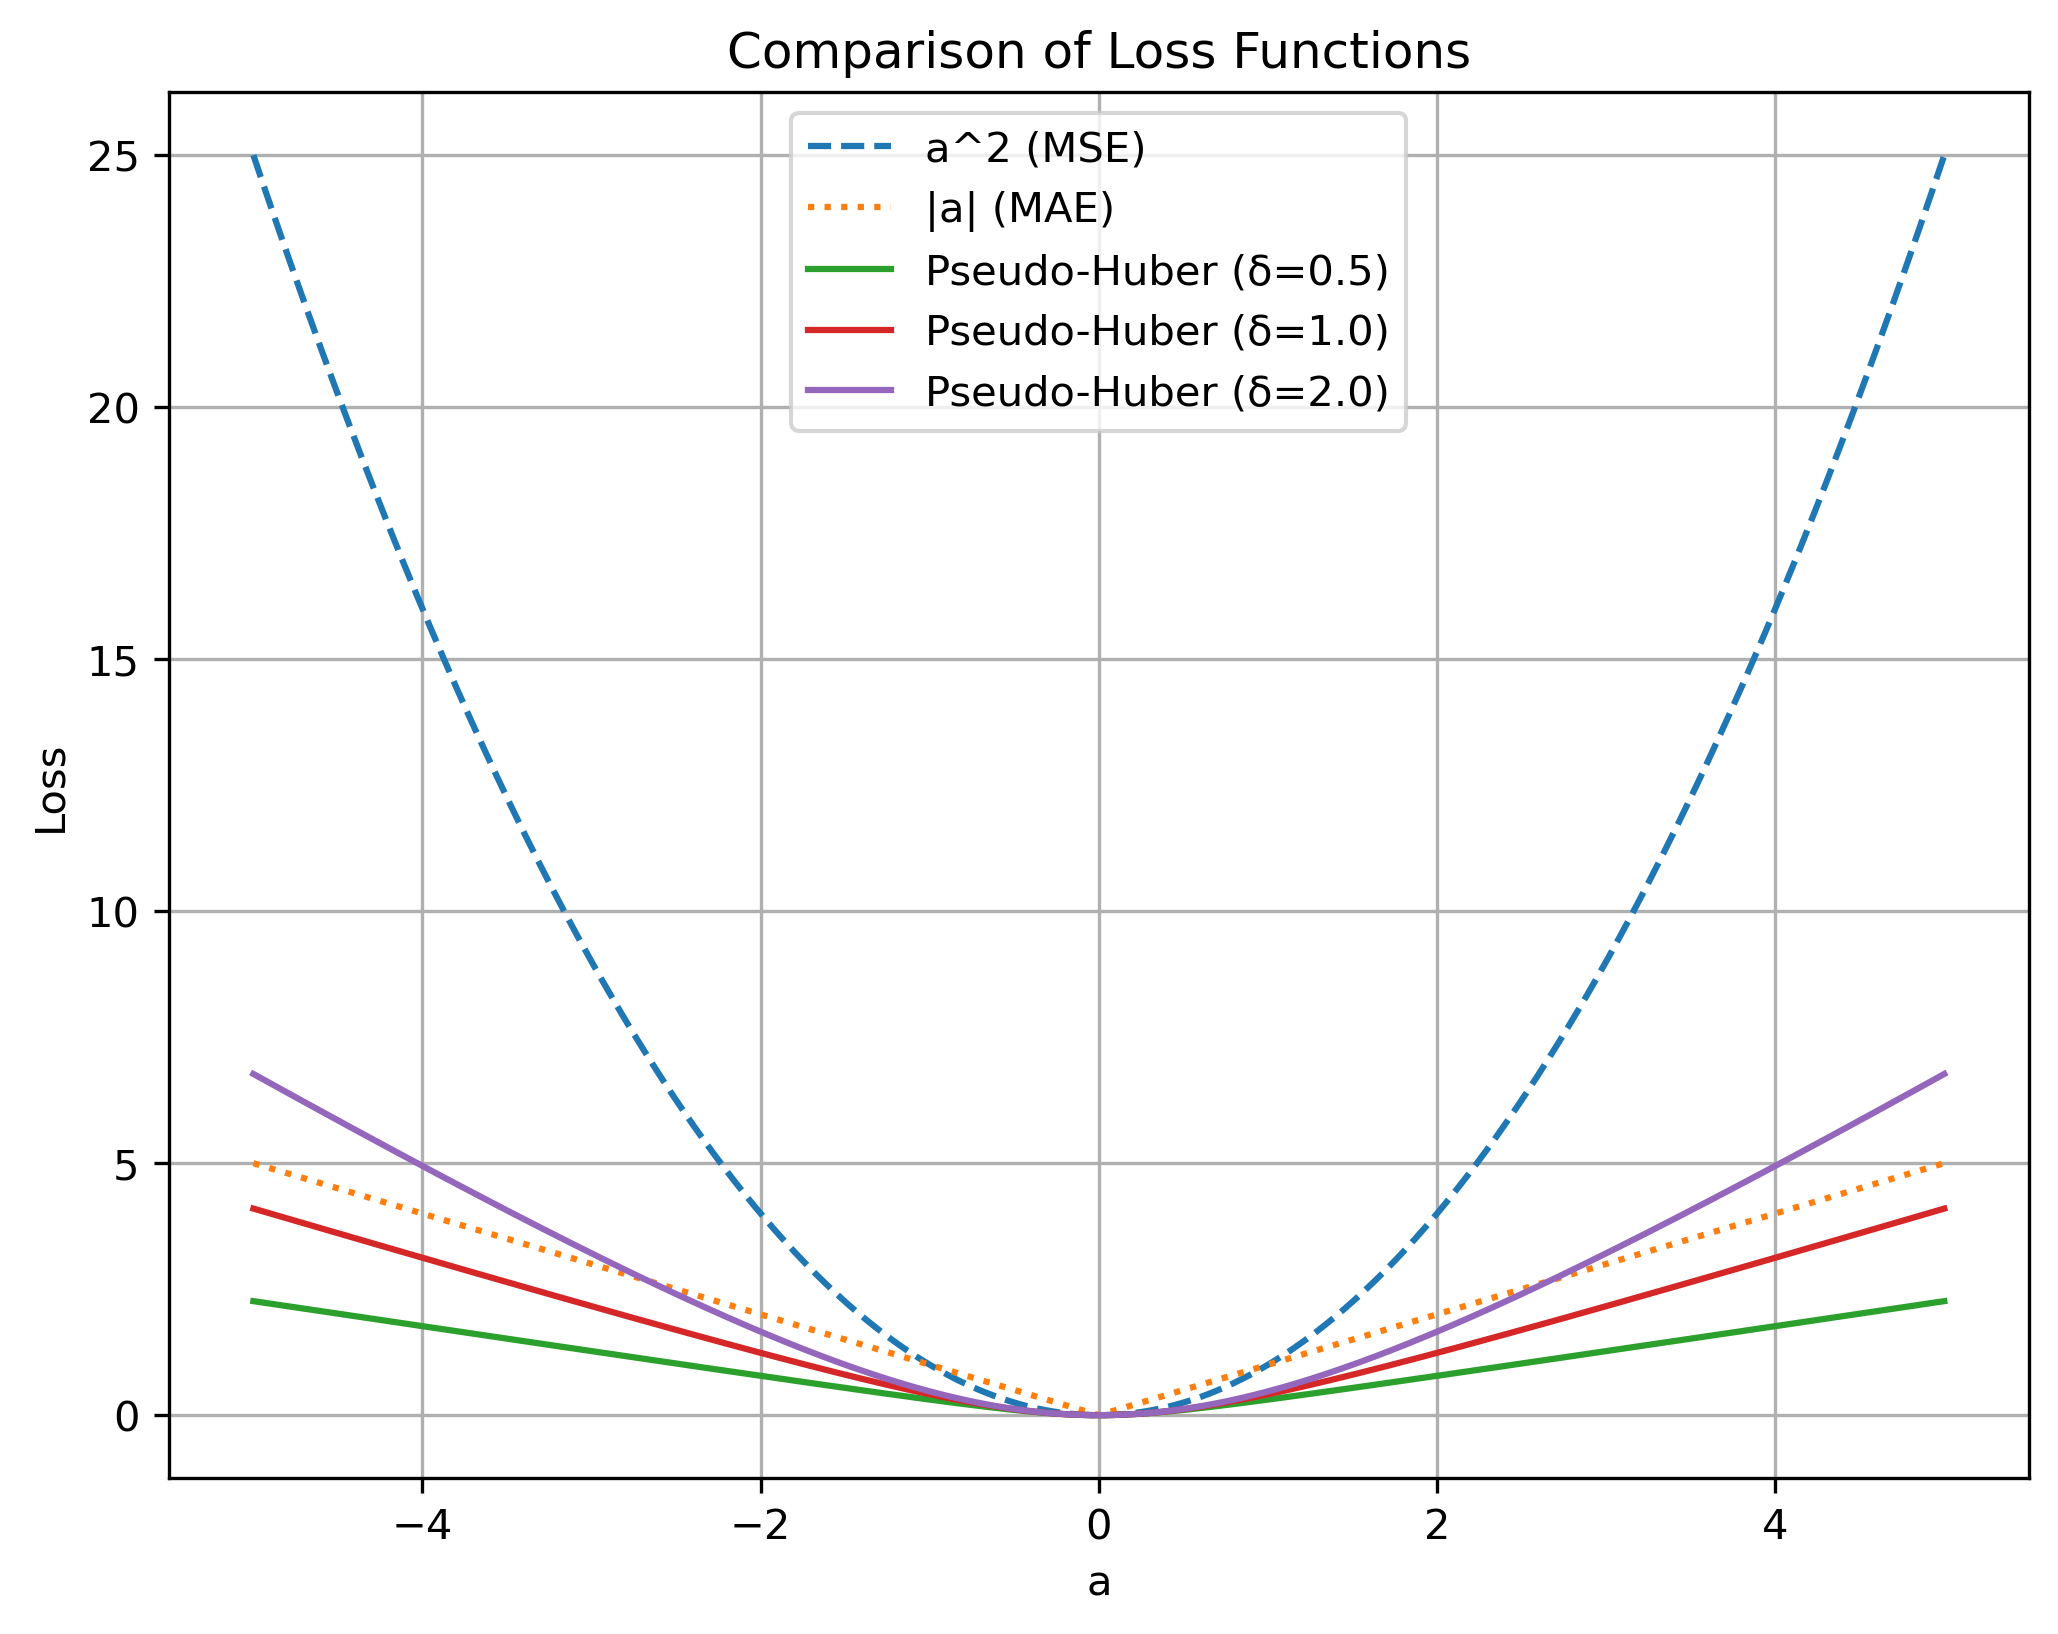
\includegraphics[width=0.7\linewidth]{plots/pseudo_huber_plot.png}
	\caption{Comparison of MSE, MAE, and Pseudo-Huber loss for different values of $\delta$.}
\end{figure}

For small values of $a$, the Pseudo-Huber loss behaves like a quadratic function:
\[
L_{\delta}(a) \approx \frac{1}{2}a^2.
\]
So near zero it is smooth and behaves similarly to MSE.

For large values of $a$, the Pseudo-Huber loss behaves approximately linearly:
\[
L_{\delta}(a) \approx \delta |a|.
\]
So for large errors it behaves more like MAE and grows much more slowly than $a^2$.

The parameter $\delta$ controls how quickly the function changes from quadratic behavior to linear behavior. Smaller $\delta$ makes the loss look more like MAE sooner, while larger $\delta$ makes it look more like MSE over a wider range.

\begin{enumerate}[label=\textbf{1(\alph*)}, start=6]
    \item Implement the loss function instead of the MSE using a custom loss function and allowing the autograd to compute the derivatives.
\end{enumerate}

Note: Refer to \href{https://docs.pytorch.org/tutorials/beginner/pytorch_with_examples.html}{PyTorch with Examples link} to the autograd example. Also, if you want to learn more about autograd (beyond this problem), refer to \href{https://docs.pytorch.org/tutorials/beginner/introyt/autogradyt_tutorial.html}{PyTorch link} for a detailed example for autograd.

\textbf{Solution}

\textbf{Code:}
\begin{lstlisting}[language=Python]
	# -*- coding: utf-8 -*-
	import torch
	import math
	
	dtype = torch.float
	device = torch.accelerator.current_accelerator().type if torch.accelerator.is_available() else "cpu"
	print(f"Using {device} device")
	torch.set_default_device(device)
	
	x = torch.linspace(-math.pi, math.pi, 2000, dtype=dtype)
	y = torch.sin(x)
	
	a = torch.randn((), dtype=dtype, requires_grad=True)
	b = torch.randn((), dtype=dtype, requires_grad=True)
	c = torch.randn((), dtype=dtype, requires_grad=True)
	d = torch.randn((), dtype=dtype, requires_grad=True)
	e = torch.randn((), dtype=dtype, requires_grad=True)
	f = torch.randn((), dtype=dtype, requires_grad=True)
	g = torch.randn((), dtype=dtype, requires_grad=True)
	h = torch.randn((), dtype=dtype, requires_grad=True)
	
	def pseudo_huber_loss(y_pred, y_true, delta=1.0):
	z = y_pred - y_true
	return (delta**2 * (torch.sqrt(1 + (z / delta) ** 2) - 1)).sum()
	
	delta = 1.0
	learning_rate = 1e-6
	for t in range(2000):
	y_pred = (
	a + b * x + c * x ** 2 + d * x ** 3 +
	e * x ** 4 + f * x ** 5 + g * x ** 6 + h * x ** 7
	)
	
	loss = pseudo_huber_loss(y_pred, y, delta=delta)
	
	loss.backward()
	
	with torch.no_grad():
	a -= learning_rate * a.grad
	b -= learning_rate * b.grad
	c -= learning_rate * c.grad
	d -= learning_rate * d.grad
	e -= learning_rate * e.grad
	f -= learning_rate * f.grad
	g -= learning_rate * g.grad
	h -= learning_rate * h.grad
	
	a.grad = None
	b.grad = None
	c.grad = None
	d.grad = None
	e.grad = None
	f.grad = None
	g.grad = None
	h.grad = None
	
	print(
	f"Result: y = {a.item()} + {b.item()} x + {c.item()} x^2 + {d.item()} x^3 + "
	f"{e.item()} x^4 + {f.item()} x^5 + {g.item()} x^6 + {h.item()} x^7"
	)
\end{lstlisting}

\textbf{Console Output:}
\begin{lstlisting}
	Using cuda device
	Result: y = -0.2885704040527344 + 0.5832257270812988 x + -0.08558587729930878 x^2 + 0.8216661214828491 x^3 + 1.0416239500045776 x^4 + -0.11592603474855423 x^5 + -0.4606887698173523 x^6 + 0.21624302864074707 x^7
\end{lstlisting}

In this implementation, I replaced the MSE with the custom Pseudo-Huber loss and allowed autograd to compute the derivatives automatically using \texttt{loss.backward()}. The model successfully ran on the GPU and produced finite coefficients, showing that the custom loss function works correctly with autograd. This demonstrates that we can define new loss functions in PyTorch without manually deriving gradients.

\newpage

\textbf{Problem 2. Sigmoid Functions}

\textbf{2(a)} The sigmoid activation function is used to compute the conditional probability for a positive example as given by:
\[
p(X) = \Pr(Y = 1|X)
\]
\[
= \frac{1}{1 + e^{-(\beta_0 + \beta_1 x_1 + \cdots + \beta_p x_p)}}.
\]

Let $z = \beta_0 + \beta_1 X_1 + \cdots + \beta_p X_p$ denote the input to the activation function. The sigmoid function $\sigma(z)$ is defined by
\[
\sigma(z) = 1/(1 + e^{-z}).
\]

\begin{enumerate}[label=\roman*.]
    \item What is the value of $z$ for $p = 0.5$? Note that this is the default value for the classification rule.
    
    \textbf{Solution}
    
    We are given the sigmoid function
    \[
    \sigma(z) = \frac{1}{1 + e^{-z}}.
    \]
    We are asked to find the value of $z$ when $p = 0.5$, i.e.,
    \[
    \sigma(z) = 0.5.
    \]
    
    Solving:
    \[
    0.5 = \frac{1}{1 + e^{-z}}
    \]
    
    Multiply both sides by $(1 + e^{-z})$:
    \[
    0.5(1 + e^{-z}) = 1
    \]
    
    \[
    0.5 + 0.5 e^{-z} = 1
    \]
    
    \[
    0.5 e^{-z} = 0.5
    \]
    
    \[
    e^{-z} = 1
    \]
    
    Taking the natural logarithm:
    \[
    -z = \ln(1) = 0
    \]
    
    \[
    z = 0.
    \]
    
    \textbf{Answer:} $z = 0$.
    
    This shows that the classification boundary occurs at $z = 0$, which corresponds to the default threshold of $p = 0.5$.
    
    \item Evaluate the expression as $z \to \infty$. What can you say about the input?
    
    \textbf{Solution}
    
    We consider the sigmoid function
    \[
    \sigma(z) = \frac{1}{1 + e^{-z}}.
    \]
    
    As $z \to \infty$, we have $e^{-z} \to 0$. Therefore,
    \[
    \sigma(z) = \frac{1}{1 + e^{-z}} \to \frac{1}{1 + 0} = 1.
    \]
    
    As $z \to \infty$, the sigmoid function approaches 1. This means that the model assigns a probability close to 1 for the positive class ($Y = 1$). This implies that the input features produce a very large positive linear combination $z = \beta_0 + \beta_1 x_1 + \cdots + \beta_p x_p$, indicating strong evidence in favor of the positive class.
    
    \item Derive an expression as $z \to -\infty$. What can you say about the input?
    
    \textbf{Solution}
    
    We consider the sigmoid function
    \[
    \sigma(z) = \frac{1}{1 + e^{-z}}.
    \]
    
    As $z \to -\infty$, we have $e^{-z} \to \infty$. Therefore,
    \[
    \sigma(z) = \frac{1}{1 + e^{-z}} \to \frac{1}{1 + \infty} = 0.
    \]
    
    As $z \to -\infty$, the sigmoid function approaches 0. This means that the model assigns a probability close to 0 for the positive class ($Y = 1$). This implies that the input features produce a very large negative linear combination $z = \beta_0 + \beta_1 x_1 + \cdots + \beta_p x_p$, indicating strong evidence in favor of the negative class ($Y = 0$).
    
\end{enumerate}

\textbf{2(b)} Rewrite the input as a dot product between two vectors:
\[
z = X'^T \beta'.
\]

Give expressions for $X'$ and $\beta'$.

\textbf{Solution}

We start with
\[
z = \beta_0 + \beta_1 X_1 + \cdots + \beta_p X_p.
\]

This can be written as a dot product by including the intercept term $\beta_0$ as part of the vectors. Define
\[
X' = 
\begin{bmatrix}
	1 \\
	X_1 \\
	X_2 \\
	\vdots \\
	X_p
\end{bmatrix},
\quad
\beta' = 
\begin{bmatrix}
	\beta_0 \\
	\beta_1 \\
	\beta_2 \\
	\vdots \\
	\beta_p
\end{bmatrix}.
\]

Then,
\[
z = X'^T \beta'.
\]

$X'$ is the augmented input vector with a leading 1, and $\beta'$ is the parameter vector including the intercept term.

\textbf{2(c)} For dot products, we have
\[
\|X^T \beta'\| = \|X'^T\| \|\beta'\| \cos \phi,
\]
where $\phi$ is the angle between $X'$ and $\beta'$. Note that $\phi$ is a regular angle for 2D and 3D vectors. Beyond 3D, we can use this property to define the angle.

Given that $\beta'$ is fixed, we are interested in finding $X'$ so that the dot product is minimized or maximized.

\begin{enumerate}[label=\roman*.]
    \item For what values of $X'$ is the probability for a positive example maximized? Sketch examples in 2D.
    
    \textbf{Solution}
    
    The probability of a positive example is
    \[
    p(X) = \sigma(z) = \frac{1}{1+e^{-z}},
    \qquad z = X'^T\beta'.
    \]
    Since the sigmoid function is increasing, the probability is maximized when the dot product $X'^T\beta'$ is maximized. Using
    \[
    X'^T\beta' = \|X'\|\,\|\beta'\|\cos\phi,
    \]
    this occurs when $\cos\phi = 1$, or equivalently when $\phi = 0$. Thus $X'$ must point in the same direction as $\beta'$, so
    \[
    X' = a\beta', \qquad a>0.
    \]
    
    \textbf{Code:}
    \begin{lstlisting}[language=Python]
    	import numpy as np
    	import matplotlib.pyplot as plt
    	import os
    	
    	os.makedirs("plots", exist_ok=True)
    	
    	beta = np.array([2, 1])
    	
    	x_max1 = 0.5 * beta
    	x_max2 = 1.5 * beta
    	x_max3 = 2.5 * beta
    	x_min1 = -0.5 * beta
    	x_min2 = -1.5 * beta
    	x_other = np.array([1, -2])
    	
    	plt.figure(figsize=(7, 7))
    	
    	plt.quiver(0, 0, beta[0], beta[1], angles='xy', scale_units='xy', scale=1, label="beta'")
    	plt.quiver(0, 0, x_max1[0], x_max1[1], angles='xy', scale_units='xy', scale=1, label="X' = a beta'")
    	plt.quiver(0, 0, x_max2[0], x_max2[1], angles='xy', scale_units='xy', scale=1)
    	plt.quiver(0, 0, x_max3[0], x_max3[1], angles='xy', scale_units='xy', scale=1)
    	plt.quiver(0, 0, x_min1[0], x_min1[1], angles='xy', scale_units='xy', scale=1, label="X' = -a beta'")
    	plt.quiver(0, 0, x_min2[0], x_min2[1], angles='xy', scale_units='xy', scale=1)
    	plt.quiver(0, 0, x_other[0], x_other[1], angles='xy', scale_units='xy', scale=1, label="other X'")
    	
    	plt.xlim(-6, 6)
    	plt.ylim(-6, 6)
    	plt.axhline(0)
    	plt.axvline(0)
    	plt.grid(True)
    	plt.gca().set_aspect('equal', adjustable='box')
    	plt.title("2D Sketch of X' and beta'")
    	plt.xlabel("x1")
    	plt.ylabel("x2")
    	plt.legend()
    	
    	plt.savefig("plots/problem2c_sketch.png", dpi=300, bbox_inches="tight")
    	plt.show()
    \end{lstlisting}
    
    \begin{figure}[H]
    	\centering
    	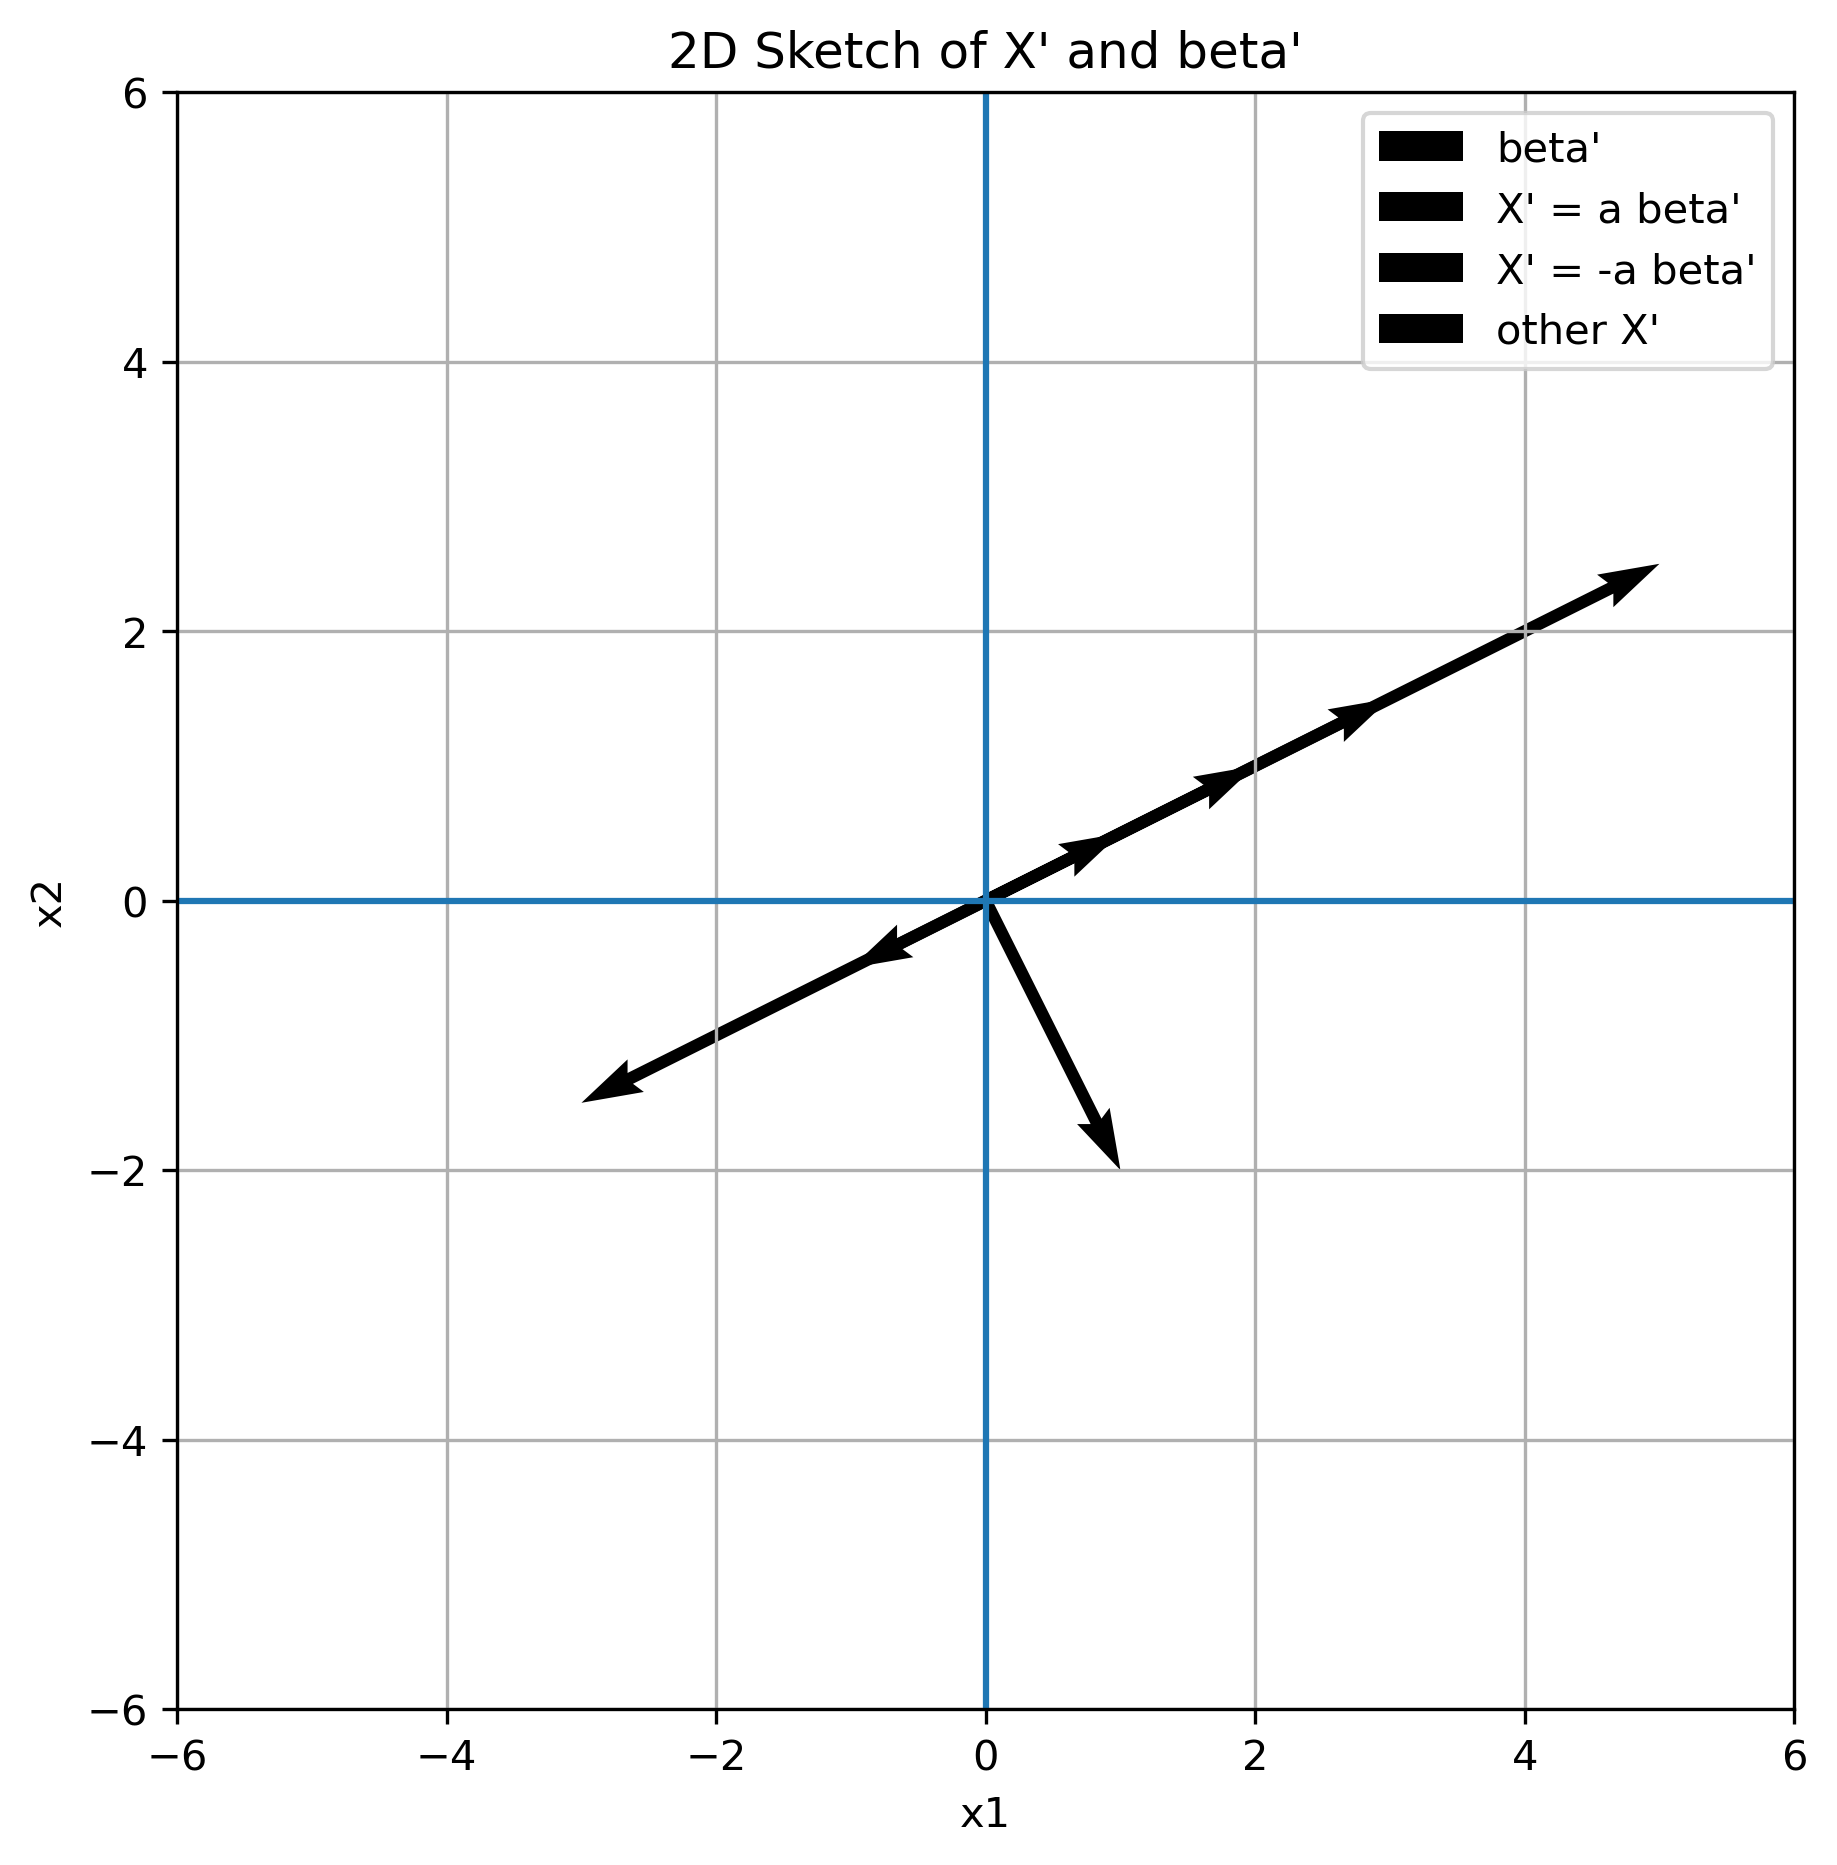
\includegraphics[width=0.7\linewidth]{plots/problem2c_sketch.png}
    	\caption{In 2D, the probability of a positive example is maximized when $X'$ points in the same direction as $\beta'$.}
    \end{figure}
    
    \item For what values of $X'$ is the probability for a negative example minimized? Sketch examples in 2D.
    
    \textbf{Solution}
    
    The probability of a negative example is
    \[
    \Pr(Y=0\mid X)=1-\sigma(z), \qquad z=X'^T\beta'.
    \]
    Since $\sigma(z)$ is increasing, $1-\sigma(z)$ is minimized when $z$ is maximized. Thus we maximize the dot product
    \[
    X'^T\beta'=\|X'\|\,\|\beta'\|\cos\phi,
    \]
    which occurs when $\cos\phi=1$ (i.e., $\phi=0$). Therefore,
    \[
    X' = a\beta', \qquad a>0.
    \]
    
    \begin{figure}[H]
    	\centering
    	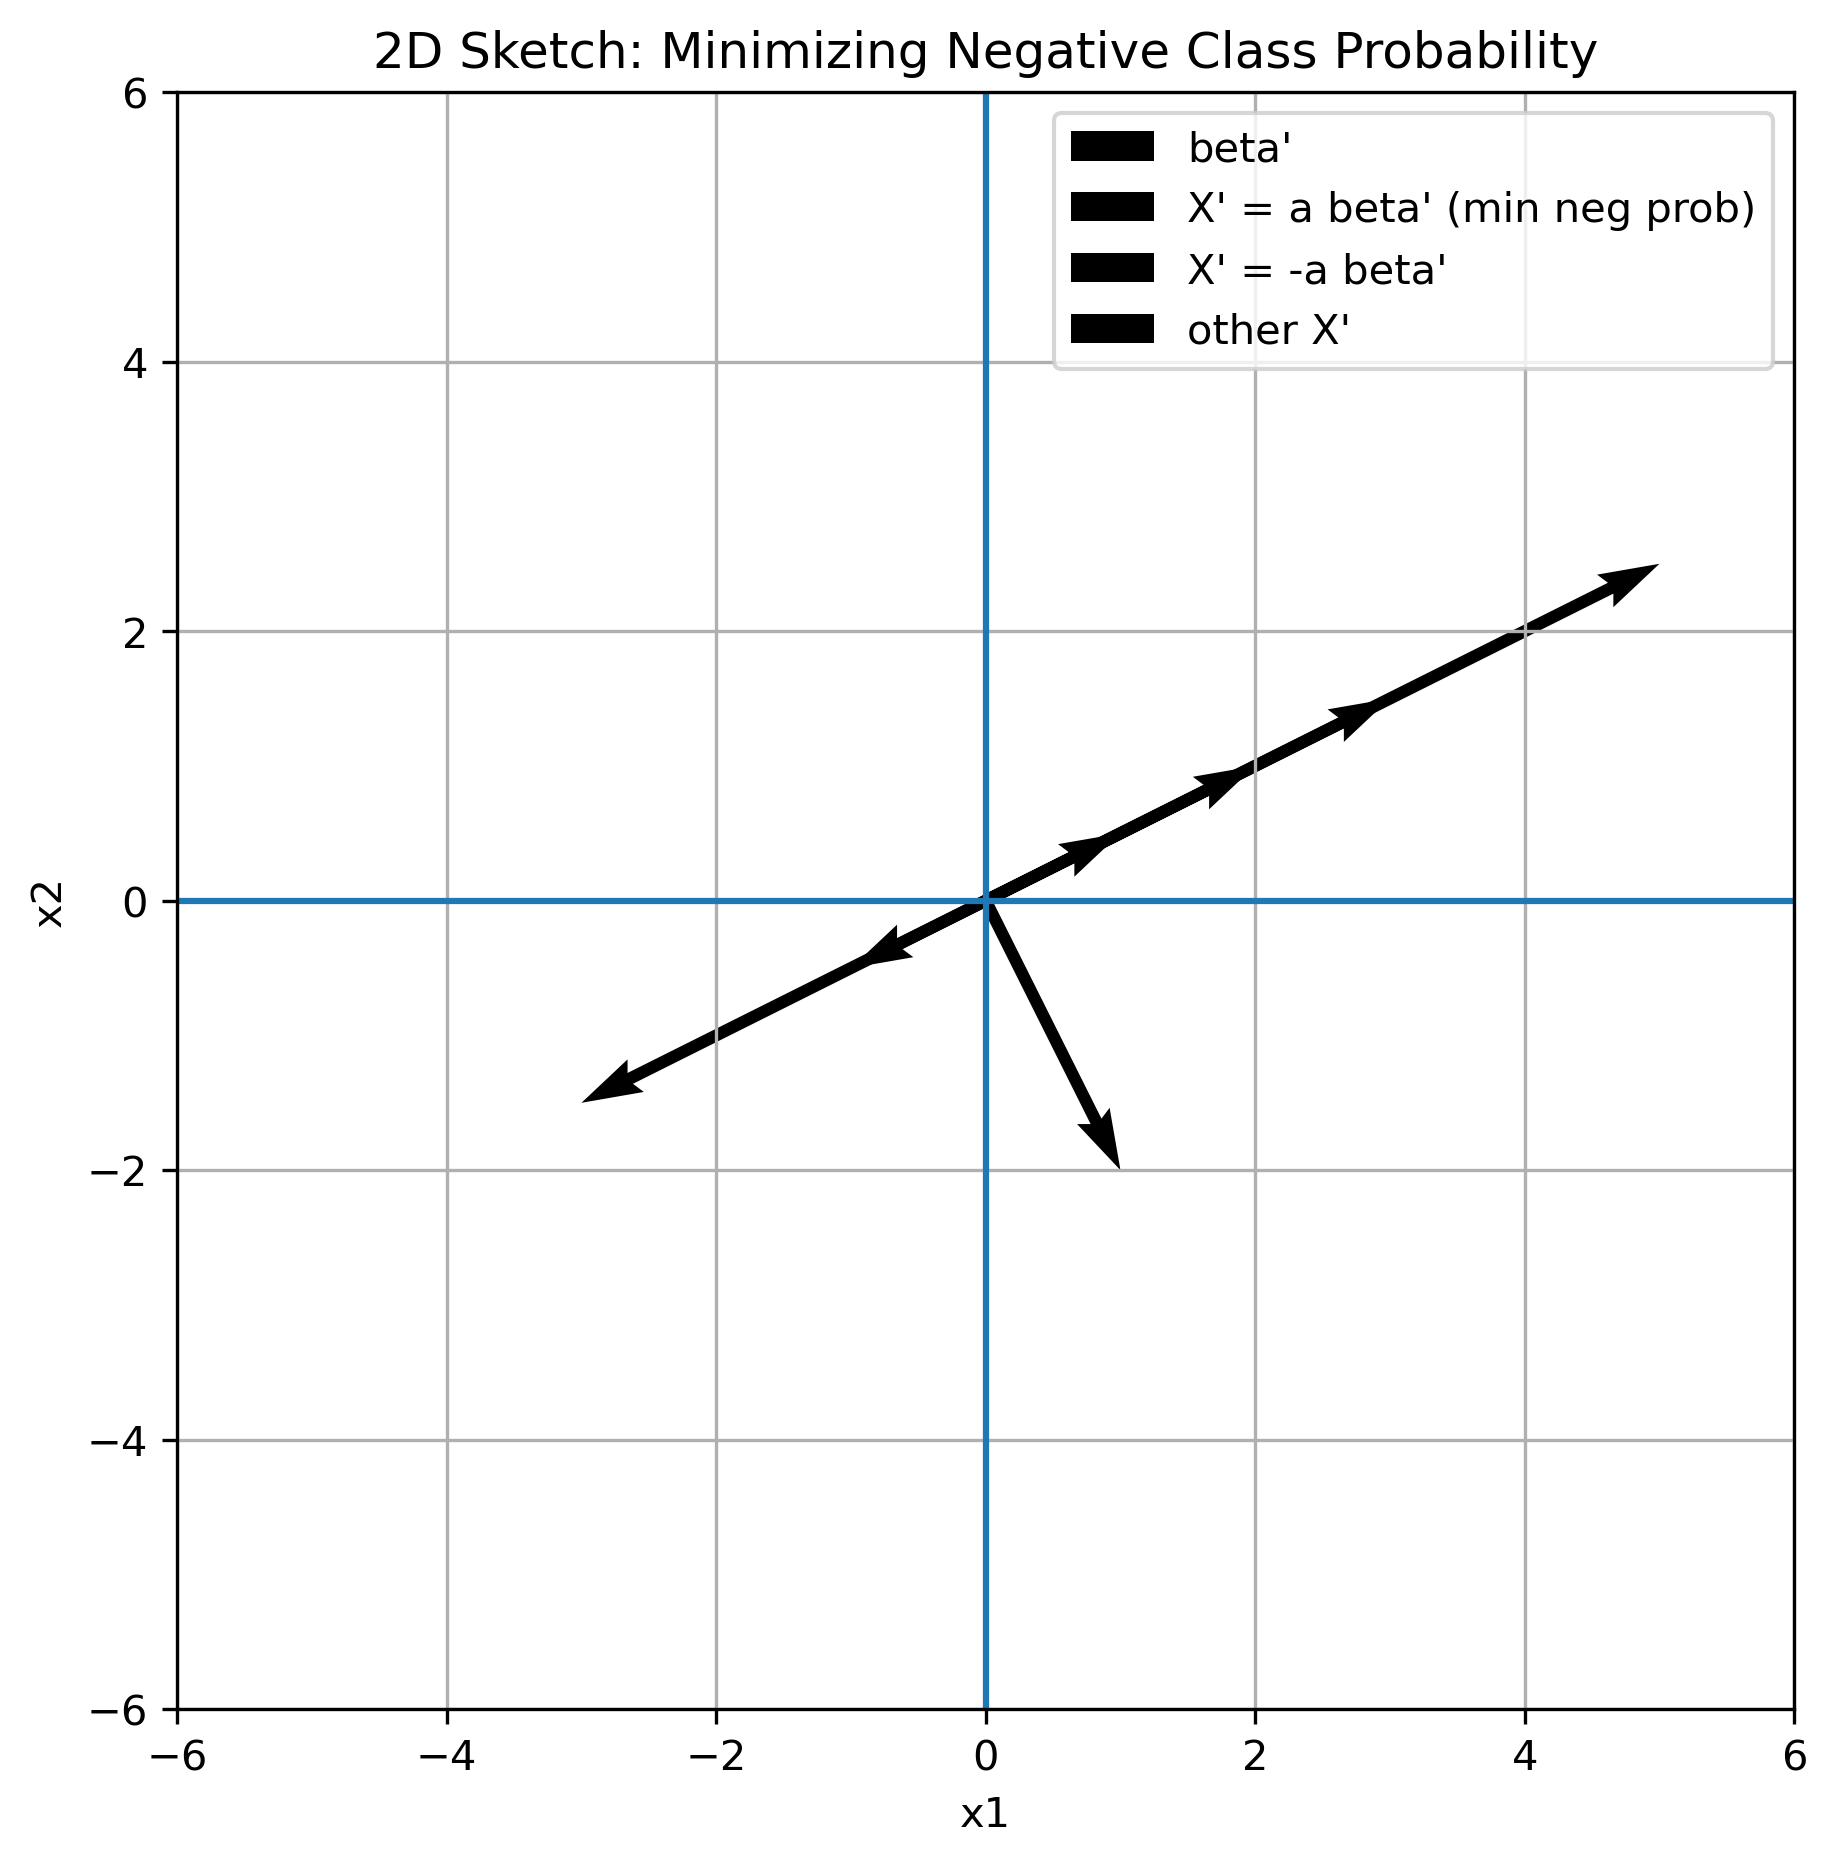
\includegraphics[width=0.7\linewidth]{plots/problem2c_negative.png}
    	\caption{The negative class probability is minimized when $X'$ points in the same direction as $\beta'$.}
    \end{figure}
    
    \item Give an expression for the values of $X'$ that are being ignored by the sigmoid. Sketch examples in 2D.
    
    \textbf{Solution}
    
    The sigmoid depends on
    \[
    z = X'^T\beta'.
    \]
    The values of $X'$ that are ignored by the sigmoid satisfy
    \[
    X'^T\beta' = 0.
    \]
    For these inputs, we have $z = 0$, and thus
    \[
    \sigma(0) = \frac{1}{2}.
    \]
    Therefore, these inputs lie exactly on the decision boundary and do not favor either class.
    
    Geometrically, $X'^T\beta' = 0$ means that $X'$ is orthogonal to $\beta'$. Hence, all ignored values are vectors perpendicular to $\beta'$.
    
    \begin{figure}[H]
    	\centering
    	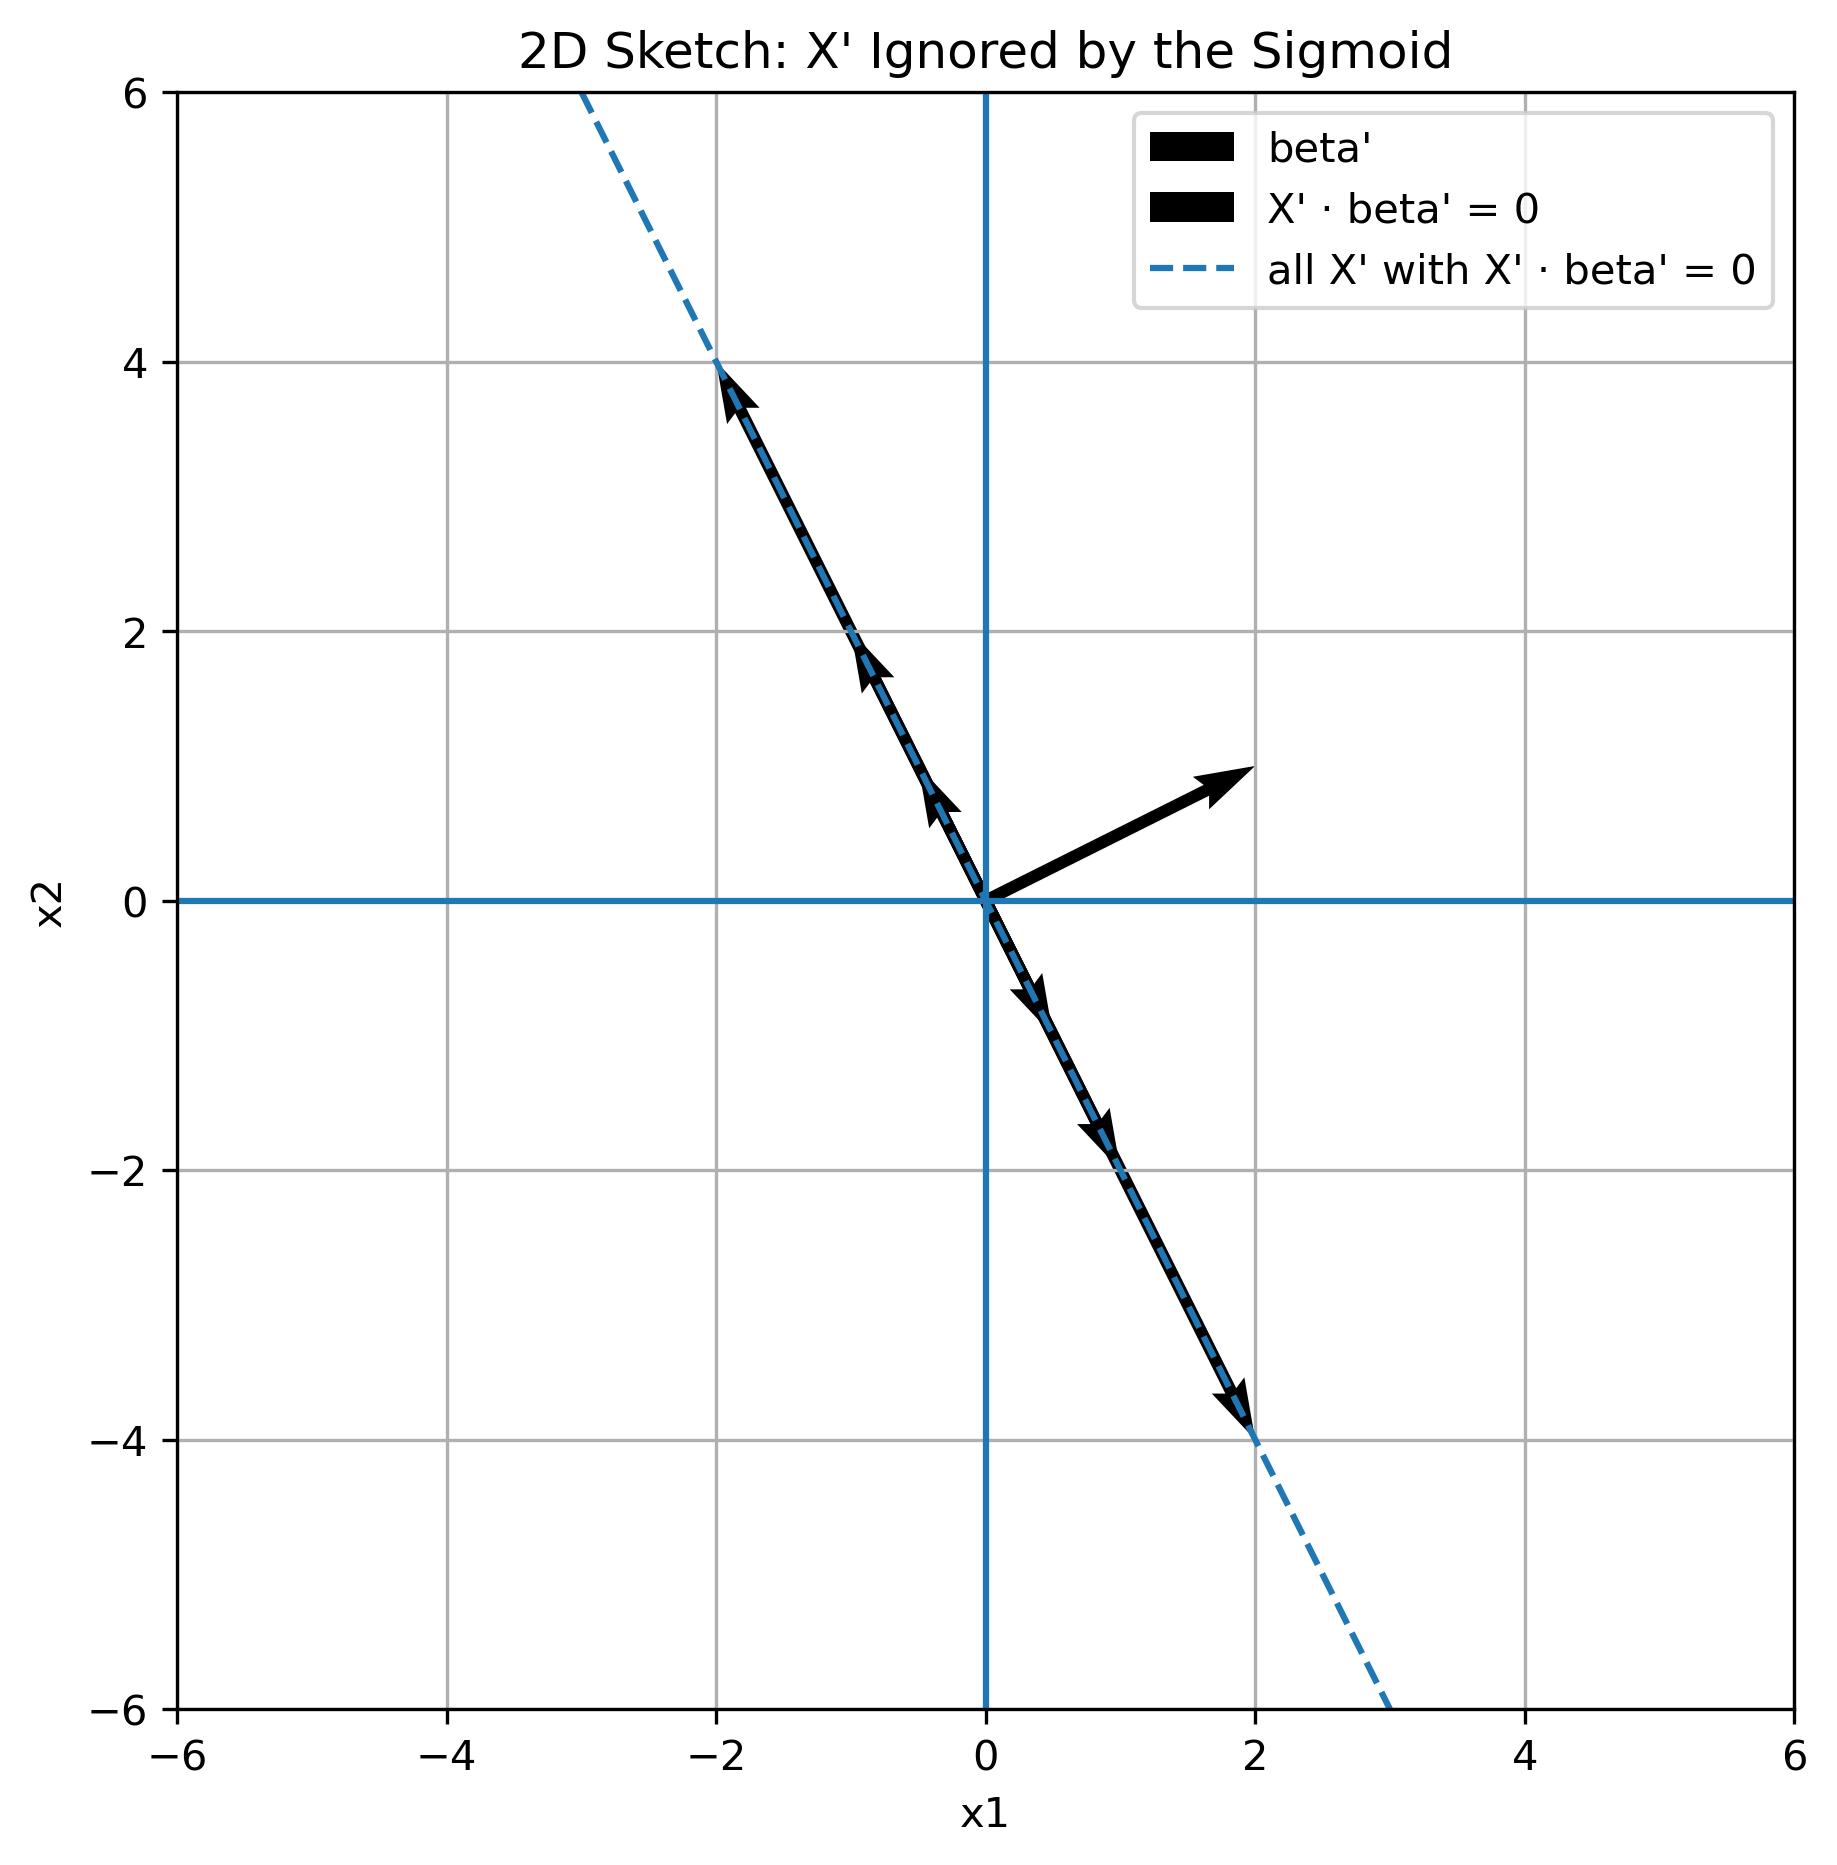
\includegraphics[width=0.7\linewidth]{plots/problem2c_ignored.png}
    	\caption{All $X'$ such that $X'^T\beta' = 0$ are perpendicular to $\beta'$ and lie on the decision boundary.}
    \end{figure}

    \textbf{Hint:} Find values of $X'$ so that $X' \cdot \beta' = 0$.
\end{enumerate}

\textbf{Additional hint:} In terms of the dot product expression, we note that we can maximize the dot product when $\phi = 0$. This happens when $X' = a\beta'$ for $a > 0$. Similarly, we get the minimum value when $X' = -a\beta'$ for $a > 0$.

\textbf{2(d)} Suppose that $X'$ corresponds to the input image. Based on your answers in 2(c), explain how you would use $\beta'$ to provide:

\begin{enumerate}[label=\roman*.]
    \item Visualize ideal positive examples.
    
    \textbf{Solution}
    
    From 2(c), the probability of a positive example is maximized when
    \[
    X' = a\beta', \qquad a>0.
    \]
    Thus, $\beta'$ itself represents the direction of an ideal positive input.
    
    If $X'$ corresponds to an image, then $\beta'$ can be reshaped into the same image dimensions. This allows us to visualize $\beta'$ directly as an “ideal positive example.” The resulting image highlights which features (pixels) contribute most strongly to predicting the positive class: large positive values indicate features that support the positive class, while negative values indicate features that oppose it.
    
    \begin{figure}[H]
    	\centering
    	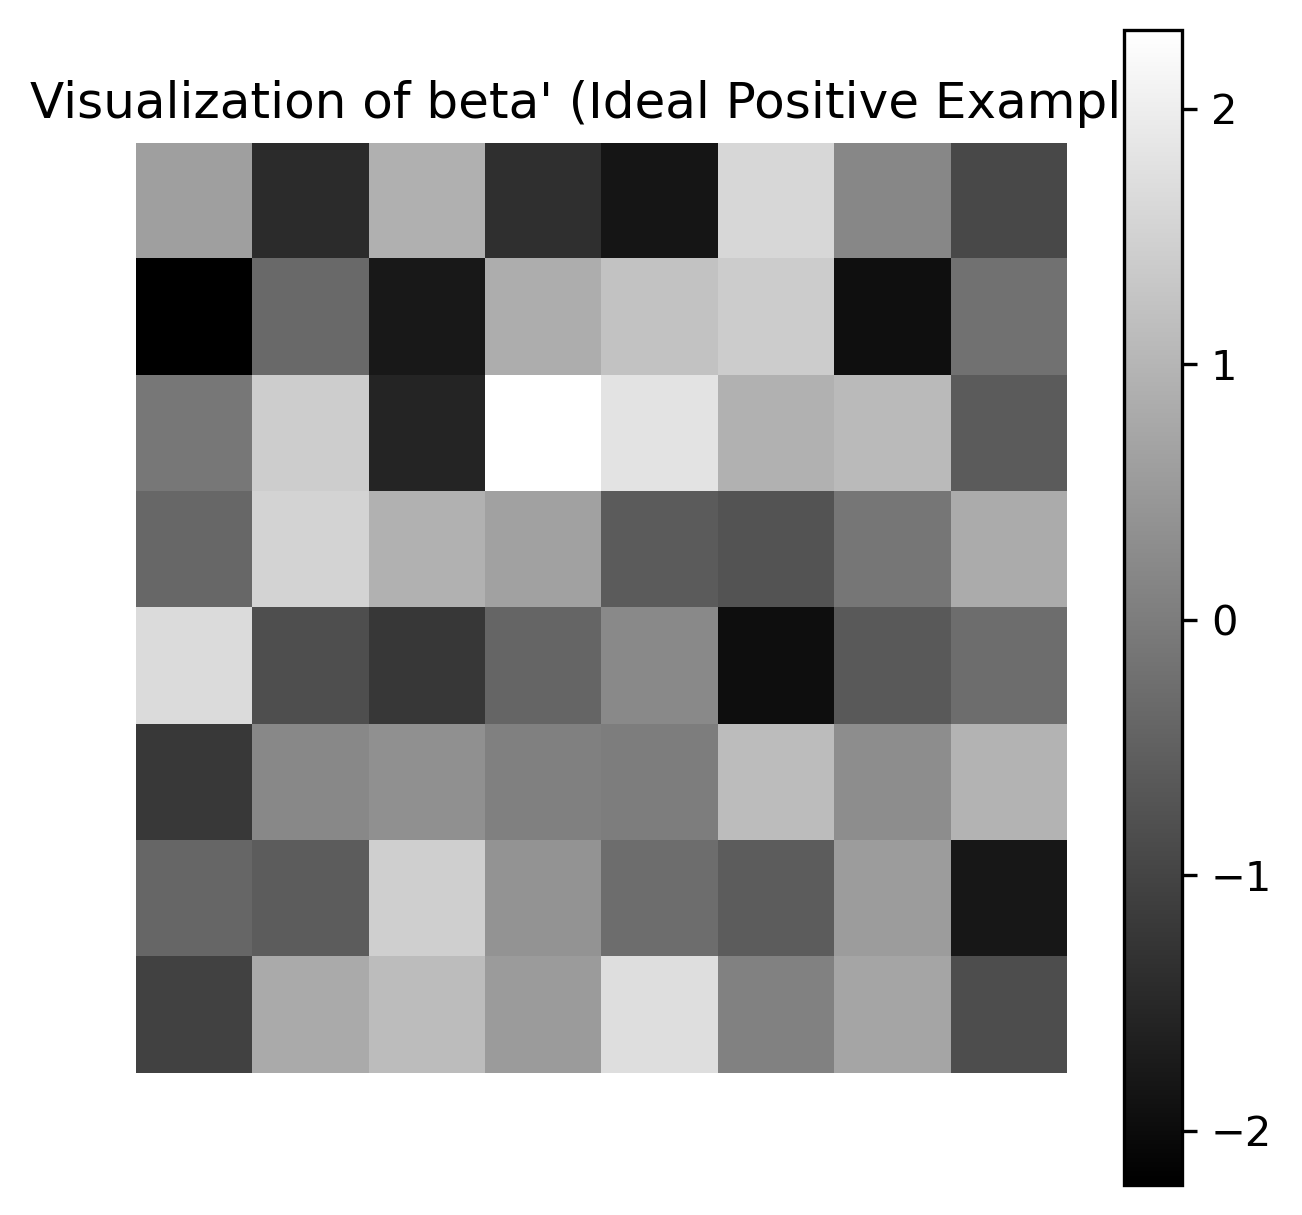
\includegraphics[width=0.5\linewidth]{plots/problem2d_beta_visualization.png}
    	\caption{Visualization of $\beta'$ reshaped as an image, representing the ideal positive example.}
    \end{figure}
    
    \item Visualize ideal negative examples.
    
    \textbf{Solution}
    
    From 2(c), the probability of a negative example is maximized when
    \[
    X' = -a\beta', \qquad a>0.
    \]
    Thus, $-\beta'$ represents the direction of an ideal negative input.
    
    If $X'$ corresponds to an image, then $-\beta'$ can be reshaped into the same image dimensions to visualize an ideal negative example. This highlights features that strongly indicate the negative class, with the sign flipped compared to $\beta'$.
    
    \begin{figure}[H]
    	\centering
    	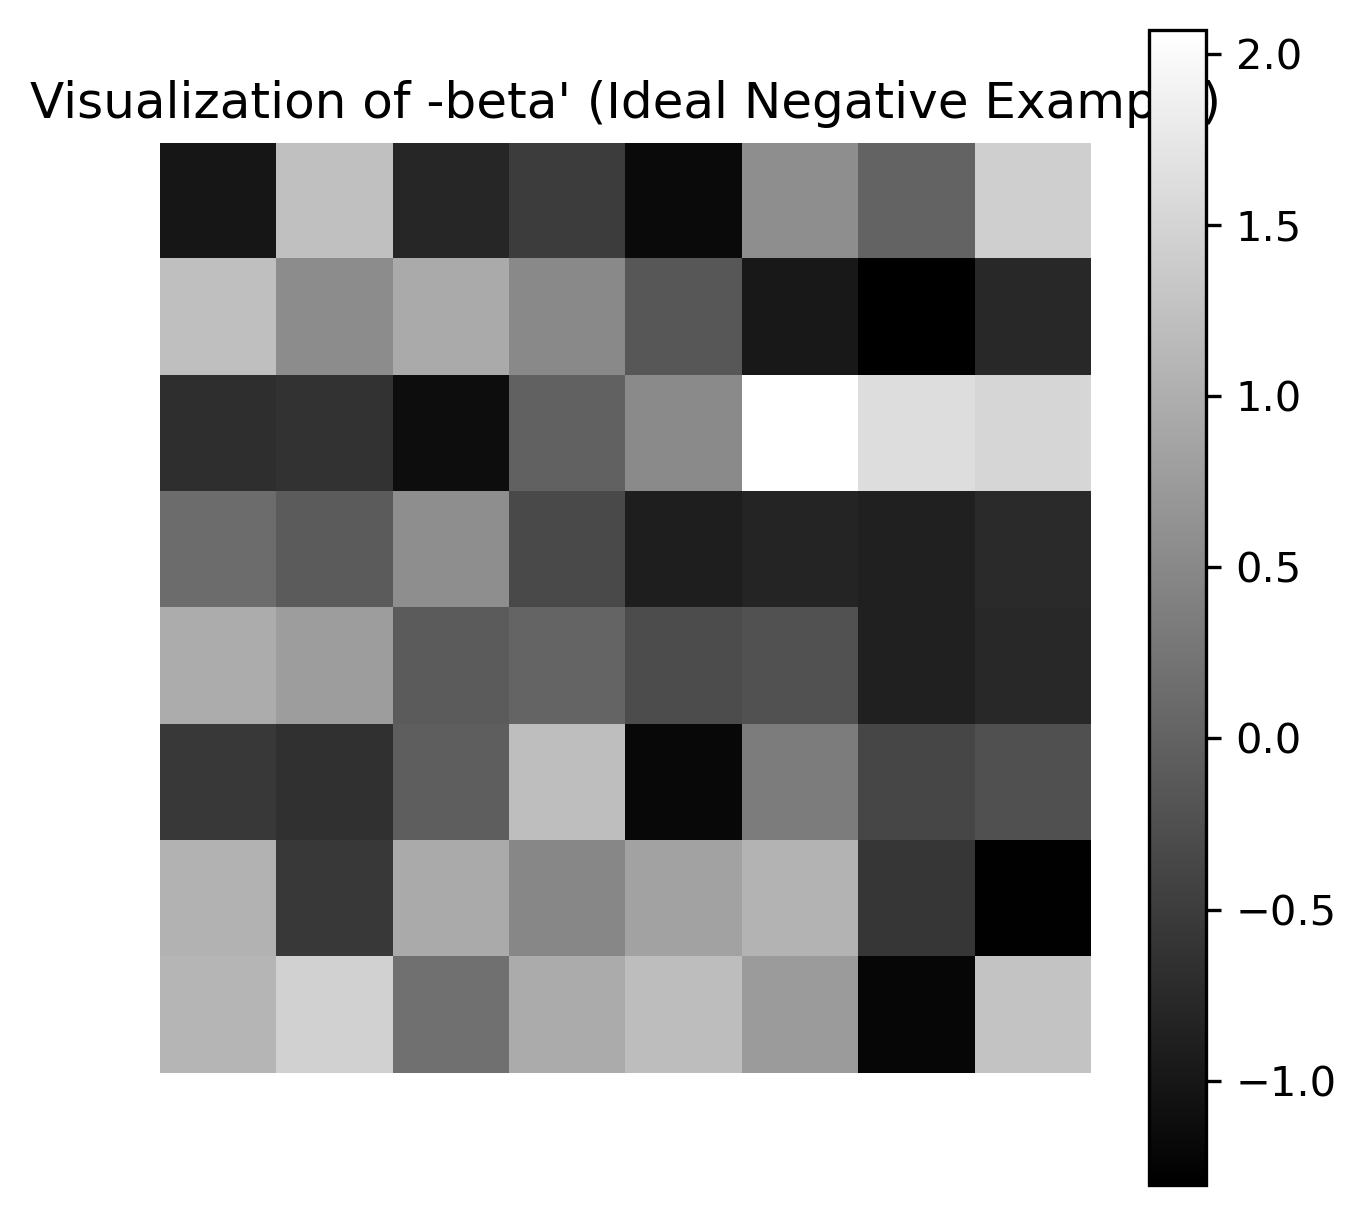
\includegraphics[width=0.5\linewidth]{plots/problem2d_beta_negative.png}
    	\caption{Visualization of $-\beta'$ reshaped as an image, representing the ideal negative example.}
    \end{figure}
    
\end{enumerate}

\textbf{2(e)} As before, assume that $X'$ corresponds to the input image. Define the residual image using Gramm-Schmitz process:
\[
R = X' - \frac{X'^T \beta'}{\beta' \beta^T}\beta
\]

Note that the residual image is orthogonal to $\beta'$. How should the residual image look like? Explain.

\textbf{Solution}

The residual image is
\[
R = X' - \frac{X'^T\beta'}{\beta'^T\beta'}\beta'.
\]
It represents the component of $X'$ that is orthogonal to $\beta'$, so
\[
R^T\beta' = 0.
\]

Thus, $R$ contains features that do not affect the classification. Visually, it should look like the parts of the image unrelated to the class (e.g., background or noise) after removing the component aligned with $\beta'$.

\newpage

\textbf{Problem 3. Tokenization.}

The code below refers to material taken from \href{https://colab.research.google.com/drive/1On-9_5LEUfJbNd3RNKE723sCWZRJeB7F?usp=sharing}{Stanford Tutorial on Transformers}. The corresponding slides come from: \href{https://docs.google.com/presentation/d/1HW0LdAc-qSF5za5Lyay201jB3sUM4PZs1agD8Wn2cUA/edit?slide=id.g3231418657f_0_259#slide=id.g3231418657f_0_259}{NLP PowerPoint presentation}.

\textbf{3(a)} Provide 3 examples of the following:
\begin{enumerate}[label=\roman*.]
    \item True positives.
    
    \textbf{Solution}
    
    A true positive occurs when the model correctly predicts a positive label:
    \[
    \hat{y} = 1 \text{ and } y = 1.
    \]
    
    \begin{enumerate}
    	\item The model predicts a sentence has positive sentiment, and it is actually positive.
    	\item The model classifies an email as spam, and it is indeed spam.
    	\item The model identifies a token as a named entity, and it is correctly a named entity.
    \end{enumerate}
    
    \item True negatives.
    
    \textbf{Solution}
    
    A true negative occurs when the model correctly predicts a negative label:
    \[
    \hat{y} = 0 \text{ and } y = 0.
    \]
    
    \begin{enumerate}
    	\item The model predicts a sentence has negative sentiment, and it is actually negative.
    	\item The model classifies an email as not spam, and it is indeed not spam.
    	\item The model identifies a token as not a named entity, and it is correctly not a named entity.
    \end{enumerate}
    
    \item False positives.
    
    \textbf{Solution}
    
    A false positive occurs when the model incorrectly predicts a positive label:
    \[
    \hat{y} = 1 \text{ and } y = 0.
    \]
    
    \begin{enumerate}
    	\item The model predicts a sentence has positive sentiment, but it is actually negative.
    	\item The model classifies an email as spam, but it is actually not spam.
    	\item The model identifies a token as a named entity, but it is not a named entity.
    \end{enumerate}
    
    \item False negatives.
    
    \textbf{Solution}
    
    A false negative occurs when the model incorrectly predicts a negative label:
    \[
    \hat{y} = 0 \text{ and } y = 1.
    \]
    
    \begin{enumerate}
    	\item The model predicts a sentence has negative sentiment, but it is actually positive.
    	\item The model classifies an email as not spam, but it is actually spam.
    	\item The model identifies a token as not a named entity, but it is actually a named entity.
    \end{enumerate}
    
\end{enumerate}

\textbf{Hint:} This refers to the following code:

\begin{lstlisting}
inputs = "I'm excited to learn about Hugging Face Transformers!"
tokenized_inputs = tokenizer(inputs, return_tensors="pt")
outputs = model(**tokenized_inputs)

labels = ['NEGATIVE', 'POSITIVE']
prediction = torch.argmax(outputs.logits)

print("Input:")
print(inputs)
print()

print("Tokenized Inputs:")
print_encoding(tokenized_inputs)
print()

print("Model Outputs:")
print(outputs)
print()

print(f"The prediction is {labels[prediction]}")
\end{lstlisting}

\textbf{3(b)} Answer the following from the Google Colab:
\begin{enumerate}[label=\roman*.]
    \item Why does the second token start with \#\#?
    
    \textbf{Solution}
    
    The \texttt{\#\#} prefix indicates that the token is a continuation of a word. In subword tokenization (e.g., WordPiece), tokens starting with \texttt{\#\#} are not standalone words but are attached to the previous token.
    
    \item What do the token IDs [CLS] and [SEP] stand for?
    
    \textbf{Solution}
    
    \texttt{[CLS]} stands for the classification token and is placed at the beginning of the input. It is used by the model to represent the entire sequence for classification tasks.
    
    \texttt{[SEP]} stands for the separator token and is used to separate different sentences or mark the end of the input.
    
    \item What are the associated token IDs?
    
    \textbf{Solution}
    
    The associated token IDs depend on the tokenizer vocabulary. For example, in BERT:
    \[
    \texttt{[CLS]} = 101, \qquad \texttt{[SEP]} = 102.
    \]
    
    \item What do the vectors of 1s in the attention\_mask represent?
    
    \textbf{Solution}
    
    The vectors of 1s in the \texttt{attention\_mask} indicate which tokens are valid and should be attended to by the model. A value of 1 means the token is real input, while 0 would indicate padding that should be ignored.
    
    \item Modify the input\_str using 3 very common and 3 very rare words. Report on any unusual tokenization patterns.
    
    \textbf{Solution}
    
    Common words (e.g., ``the'', ``and'', ``is'') are tokenized as single tokens, while rare words are split into multiple subword tokens with \texttt{\#\#} prefixes.
    
    Rare words are broken into smaller known subwords, leading to longer token sequences.
    
    \item Enter multiple phrases to the tokenizer. Examine the code. How is the attention map affected by padding?
    
    \textbf{Solution}
    
    When multiple phrases are tokenized together, shorter phrases are padded so that all sequences have the same length. The \texttt{attention\_mask} assigns 1 to real tokens and 0 to padding tokens. Padding positions are ignored by the model, so they do not contribute to attention.
    
\end{enumerate}

\textbf{3(c)} Consider the multilayer multihead example given in Google Colab. Answer the following:
\begin{enumerate}[label=\roman*.]
    \item What is the number of layers? What is the input layer? What is the output layer?
    \item How does "!" affect classification? To describe the relationship, you need to specify the layer and head map for your discussion.
    \item Which maps seem to respond to the sequencing of tokens (e.g., relating to the next token)? Explain.
    \item Which maps seem to correspond to preserving the ordering of the tokens (e.g., relating to themselves)? Explain.
    \item Do the relationships between [SEP] and the rest of the tokens make sense? Why or why not?
\end{enumerate}

\textbf{3(d)} Explain every number and every parameter value in the following code:

\begin{lstlisting}
prompt = "Once upon a time"

tokenized_prompt = gpt2_tokenizer(prompt, return_tensors="pt")

for i in range(10):
    output = gpt2.generate(**tokenized_prompt,
                           max_length=50,
                           do_sample=True,
                           top_p=0.9)

    print(f"{i + 1}) {gpt2_tokenizer.batch_decode(output)[0]}")
\end{lstlisting}

\textbf{Solution}

\begin{itemize}
	\item \texttt{prompt = "Once upon a time"}: The initial text used as input to generate new tokens.
	
	\item \texttt{return\_tensors="pt"}: Converts the tokenized input into PyTorch tensors.
	
	\item \texttt{for i in range(10)}: Runs the generation 10 times to produce 10 different outputs.
	
	\item \texttt{i + 1}: Used to label outputs starting from 1 instead of 0.
	
	\item \texttt{max\_length=50}: The maximum total number of tokens (input + generated) in the output sequence.
	
	\item \texttt{do\_sample=True}: Enables random sampling instead of always choosing the most probable next token.
	
	\item \texttt{top\_p=0.9}: Uses nucleus (top-p) sampling, selecting from the smallest set of tokens whose cumulative probability is at least 0.9.
	
	\item \texttt{gpt2.generate(**tokenized\_prompt)}: Generates new text based on the input prompt.
	
	\item \texttt{gpt2\_tokenizer.batch\_decode(output)}: Converts generated token IDs back into readable text.
	
	\item \texttt{[0]}: Extracts the generated sequence from the batch output.
\end{itemize}

\textbf{3(e)} Set do-sample=False and discuss the results.

\textbf{Solution}

Setting \texttt{do\_sample=False} uses greedy decoding, so the model always chooses the most probable next token at each step.

\textbf{Console Output:}
\begin{lstlisting}
	1) Once upon a time, the world was a place of great beauty and great danger. The world was a place of great danger, and the world was a place of great danger. The world was a place of great danger, and the world was a
	2) Once upon a time, the world was a place of great beauty and great danger. The world was a place of great danger, and the world was a place of great danger. The world was a place of great danger, and the world was a
	3) Once upon a time, the world was a place of great beauty and great danger. The world was a place of great danger, and the world was a place of great danger. The world was a place of great danger, and the world was a
	4) Once upon a time, the world was a place of great beauty and great danger. The world was a place of great danger, and the world was a place of great danger. The world was a place of great danger, and the world was a
	5) Once upon a time, the world was a place of great beauty and great danger. The world was a place of great danger, and the world was a place of great danger. The world was a place of great danger, and the world was a
	6) Once upon a time, the world was a place of great beauty and great danger. The world was a place of great danger, and the world was a place of great danger. The world was a place of great danger, and the world was a
	7) Once upon a time, the world was a place of great beauty and great danger. The world was a place of great danger, and the world was a place of great danger. The world was a place of great danger, and the world was a
	8) Once upon a time, the world was a place of great beauty and great danger. The world was a place of great danger, and the world was a place of great danger. The world was a place of great danger, and the world was a
	9) Once upon a time, the world was a place of great beauty and great danger. The world was a place of great danger, and the world was a place of great danger. The world was a place of great danger, and the world was a
	10) Once upon a time, the world was a place of great beauty and great danger. The world was a place of great danger, and the world was a place of great danger. The world was a place of great danger, and the world was a
\end{lstlisting}

All outputs are identical and highly repetitive, showing that greedy decoding produces deterministic and less diverse text.

\textbf{3(f)} Set top-p=0.1 and discuss the results.

\textbf{Solution}

Setting \texttt{top\_p = 0.1} restricts sampling to only a very small set of high-probability tokens.

\textbf{Console Output:}
\begin{lstlisting}
	1) Once upon a time, the world was a place of great beauty and great danger. The world was a place of great danger, and the world was a place of great danger. The world was a place of great danger, and the world was a
	2) Once upon a time, the world was a place of great beauty and great danger. The world was a place of great danger, and the world was a place of great danger. The world was a place of great danger, and the world was a
	3) Once upon a time, the world was a place of great beauty and great danger. The world was a place of great danger, and the world was a place of great danger. The world was a place of great danger, and the world was a
	4) Once upon a time, the world was a place of great beauty and great danger. The world was a place of great danger, and the world was a place of great danger. The world was a place of great danger, and the world was a
	5) Once upon a time, the world was a place of great beauty and great danger. The world was a place of great danger, and the world was a place of great danger. The world was a place of great danger, and the world was a
	6) Once upon a time, the world was a place of great beauty and great danger. The world was a place of great danger, and the world was a place of great danger. The world was a place of great danger, and the world was a
	7) Once upon a time, the world was a place of peace and harmony. But now, the world is a place of war and chaos. The world is a place of war and chaos. The world is a place of war and chaos. The world
	8) Once upon a time, the world was a place of great beauty and great danger. The world was a place of great danger, and the world was a place of great danger. The world was a place of great danger, and the world was a
	9) Once upon a time, the world was a place of great beauty and great danger. The world was a place of great danger, and the world was a place of great danger. The world was a place of great danger, and the world was a
	10) Once upon a time, the world was a place of great beauty and great danger. The world was a place of great danger, and the world was a place of great danger. The world was a place of great danger, and the world was a
\end{lstlisting}

The outputs are still very similar across runs, with only slight variation. This shows that \texttt{top\_p = 0.1} makes generation highly restrictive, so the text is less diverse and more repetitive.

\textbf{3(g)} Set top-p=0.99 and discuss the results.

\textbf{Solution}

Setting \texttt{top\_p = 0.99} allows sampling from a much larger set of likely tokens.

\textbf{Console Output:}
\begin{lstlisting}
	1) Once upon a time of darkness, the King of Nergal went out in search of a hidden way of the land. He was a young man from a young age who had never been seen in his life: long as he held forth his sword
	2) Once upon a time he had fallen in love, only to return with a girl. She told him of the two boys that he had killed her two years earlier. He then took her and turned her in for torture, and then he was beaten,
	3) Once upon a time a person might be thought of as a person only, the power of the Lord Christ to unite all the believers into one Godhead in heaven would be so great that we might not be capable of the work that one would have under
	4) Once upon a time, when the majority was, as John Marshall once said, "very far from being the first thing to go to the table after they cut all of the throats," they were not quite ready for "the other" when we come
	5) Once upon a time the three of us were walking together, sitting quietly together, listening to a song. And it was very interesting to us. We were all so excited, so excited, so excited. It was kind of exciting, to have a
	6) Once upon a time, it can be seen that people believe that a woman's body and her fertility is somehow more important than her genitals. Or, perhaps the fact that women are more likely than men to be born with the "good genes" of
	7) Once upon a time, during the life of the king that is known as a "King," were there persons ever known to give life to something like that. From a little distance, we are sure that is how the story was told at King's
	8) Once upon a time, it would appear I was in the middle of something I never imagined I should be in. When I got home from home I found the bathroom at the front of the house, a box of clothes on it. For some reason
	9) Once upon a time a new generation of leaders has arisen to lead the planet. The Earth is being transformed by this evolution. The human race has finally become a modern democracy. As long as capitalism and the state maintain control of the economy, the political
	10) Once upon a time, they were going to need these in the form of a small dose, perhaps a tablespoon. At that time the main problems of those times were to get the best dosage, rather than to get a very large dosage, and that
\end{lstlisting}

\textbf{Observation:} The outputs are much more varied across runs than with \texttt{top\_p = 0.1}. This makes the text more diverse and creative, but some outputs are less coherent and feel more random.

\textbf{Problem 4. Basic transformer architecture.}

For tutorials on convolutional and linear layers, refer to \href{https://github.com/pattichis/AIML}{AIML tutorials}. Basic training and testing is described in \href{https://colab.research.google.com/github/pattichis/AIML/blob/main/Session_16_models.ipynb}{CNN and linear models in Python}. Note that the use of nn.Parameter(.) makes parameters learnable.

For (a)-(c), refer to: \href{https://colab.research.google.com/drive/1T1-v3hXGcXqsljqvuRmXmlGUBS7qYo_b?usp=sharing}{Part 15 transformers for nlp and chatbots.ipynb}. For the ViT and DINO problems, refer to: \href{https://colab.research.google.com/drive/1gFiqft0ngNU7nIxpqfbfJ94XhnSdju5u?usp=sharing}{Fixed 16 vision and multimodal transformers.ipynb}

{\color{blue} This problem is worth 3 times as much credit as all other problems.}

\textbf{4(a)} For each of the models below, you need to provide the following:

\begin{enumerate}[label=\alph*.]
    \item Input dimensions.
    \item Output dimensions.
    \item Equation of what is being implemented. Feel free to refer to earlier parts here. For example, define the encoder and decoder in terms of the input layers.
    \item List learnable parameters.
\end{enumerate}

Here is the list of models:
\begin{enumerate}[label=\roman*.]
    \item TransformerEncoderLayer
    \item TransformerDecoderLayer
    \item TransformerEncoder
    \item TransformerDecoder
    \item MultiheadAttention
    \item Transformer
\end{enumerate}

\textbf{4(b)} Describe briefly how the NmtTransformer is trained.

For this problem, you need to provide

\begin{enumerate}[label=\alph*.]
    \item What are the inputs used for training?
    \item What is the optimizer? How is the optimizer set up?
    \item How many epochs are used for training?
\end{enumerate}

\textbf{4(c)} Describe briefly how the NmtTransformer is deployed.

\begin{enumerate}[label=\alph*.]
    \item What are the inputs and computed outputs?
    \item How is the transformer connecting the decoder to the encoder for computing outputs?
\end{enumerate}
\textbf{4(d)} For each of the models below, you need to provide the following:

\begin{enumerate}[label=\alph*.]
    \item Input dimensions
    \item Output dimensions
    \item Equation of what is being implemented. Feel free to refer to earlier parts here. For example, define the encoder and decoder in terms of the input layers.
\end{enumerate}

Here is the list of models:
\begin{enumerate}[label=\roman*.]
    \item PatchEmbedding.
    \item TransformerEncoderLayer
    \item ViT
\end{enumerate}

\textbf{4(e)} For DINO, we use two ViT systems. The teacher is trained on the full input image. The student is trained on zoomed versions of the same input image. Self distillation with no labels trains the student to produce the same output as the teacher (who is not trained). For each one of the 12 images in the DINO example in the code, comment on high attention values for image segmentation of the two cats. Specifically, highlight image regions that appear:

\begin{enumerate}[label=\roman*.]
    \item correct.
    \item wrong.
    \item may be correct.
\end{enumerate}

\textbf{Problem 5. (Contrastive learning models)}

For the basics of contrastive learning, refer to \href{https://lightning.ai/docs/pytorch/1.8.1/notebooks/course_UvA-DL/13-contrastive-learning.html}{Self-supervised contrastive learning with SIMCLR}.

For the CLIP problem, refer to: \href{https://colab.research.google.com/drive/1gFiqft0ngNU7nIxpqfbfJ94XhnSdju5u?usp=sharing}{Fixed 16 vision and multimodal transformers.ipynb}.

\textbf{5(a)} Based on the example with SIMCLR, for this problem, refer to contrast\_transforms. Provide pseudocode to expand the list of possible transforms for:

\begin{enumerate}[label=\roman*.]
    \item A bigger variety of scalings.
    \item Different color variations.
    \item Different bluring functions.
\end{enumerate}

\textbf{5(b)} Explain how the following transformations may not work for contrastive learning:

\begin{enumerate}[label=\roman*.]
    \item Random resizing.
    \item Random resized cropping.
\end{enumerate}

\textbf{5(c)} Evaluate the InfoNCE loss for:

\begin{enumerate}[label=\roman*.]
    \item Ideal cases for N=2 and N=1000, temperature=1.
    \item Ideal cases for N=2 and N=1000, temperature=100.
    \item Ideal cases for N=2 and N=1000, temperature=0.1.
    \item Realistic cases for maximum score=0.9, minimum score=0, N=2, and N=1000, with temperature=1.
    \item Realistic cases for maximum score=0.9, minimum score=0, N=2, and N=1000, with temperature=0.1.
    \item Realistic cases for maximum score=0.9, minimum score=0, N=2, and N=1000, with temperature=100.
\end{enumerate}

Discuss the effect of changing the temperature.

\textbf{5(d)} Provide a block diagram showing the architecture for pre-training.

\textbf{5(e)} Provide a block diagram showing the architecture for classification.

\textbf{5(f)} Consider the multimodal transformer based on CLIP. In our example, we have the following code for encoding text and images separately:

\begin{lstlisting}
similarities = image_features @ text_features.T
temperature = clip_model.logit_scale.detach().exp()
rescaled_similarities = similarities * temperature
probabilities = torch.nn.functional.softmax(rescaled_similarities , dim=1)
\end{lstlisting}

Study the high and low similarity values produced here and answer the following: Explain the following:

\begin{enumerate}[label=\roman*.]
    \item What is the ideal similarity when a generated caption corresponds to the image?
    \item What is the ideal similarity when a generated caption does not correspond to the image?
    \item What is a realistic similarity when a generated caption corresponds to the image?
    \item What is a realistic similarity when a generated caption does not correspond to the image?
\end{enumerate}

\end{document}